% for notes environment
\usepackage{xsavebox}
\usepackage{hyperref}
\usepackage{graphicx}
\usepackage{luatexja}
\usepackage[hiragino-pro,deluxe,nfssonly,jis2004]{luatexja-preset}
\usepackage{fontspec}
\usepackage{epigraph}
\usepackage{etoolbox}
\usepackage{tikz}
\usepackage{framed}
\usepackage{mathtools}
\usepackage{listings}
\usepackage{libertine}
\usepackage[libertine]{newtxmath}
\usepackage{bxcoloremoji}
\usepackage{xcolor}
\usepackage{diagbox}
\usepackage{caption}
\usepackage{appendixnumberbeamer}
\usepackage{multirow}
\usepackage{xpatch}
\usepackage{multicol}
\usepackage{tabularx}
\usepackage{bussproofs}

\newenvironment{scaledprooftree}[1]%
  {\gdef\scalefactor{#1}\begin{center}\proofSkipAmount \leavevmode}%
  {\scalebox{\scalefactor}{\DisplayProof}\proofSkipAmount \end{center} }

\usetikzlibrary{fit}

\setmonofont{CMU Typewriter Text}

\definecolor{links}{HTML}{2A1B81}
\hypersetup{colorlinks,linkcolor=,urlcolor=links}

\usetheme{Boadilla}
\usecolortheme{seahorse}
% セリフフォント
\usefonttheme{serif}

\xpatchcmd{\itemize}
  {\def\makelabel}
  {\ifnum\@itemdepth=1\relax
     \setlength\itemsep{1.2ex}% separation for first level
   \else
     \ifnum\@itemdepth=2\relax
       \setlength\itemsep{0.8ex}% separation for second level
       \setlength\topsep{1.2ex}
     \else
       \ifnum\@itemdepth=3\relax
         \setlength\itemsep{0.05ex}% separation for third level
         \setlength\topsep{0.8ex}
   \fi\fi\fi\def\makelabel
  }
 {}
 {}

\setbeamercolor{page number in head/foot}{bg=blue!10}
\setbeamertemplate{footline}{%
  \leavevmode%
  \hbox{%
    \begin{beamercolorbox}[wd=.3\paperwidth,ht=2.25ex,dp=1ex,center]{author in head/foot}%
      \usebeamerfont{author in head/foot}\insertshortauthor\hspace*{1ex}(\insertshortinstitute)
    \end{beamercolorbox}%
    \begin{beamercolorbox}[wd=.3\paperwidth,ht=2.25ex,dp=1ex,center]{title in head/foot}%
      \usebeamerfont{title in head/foot}\insertshorttitle
    \end{beamercolorbox}%
    \begin{beamercolorbox}[wd=.3\paperwidth,ht=2.25ex,dp=1ex,center]{date in head/foot}%
      \insertshortdate{} @ \InsertConferenceShort
    \end{beamercolorbox}%
    \begin{beamercolorbox}[wd=.1\paperwidth,ht=2.25ex,dp=1ex,center]{page number in head/foot}%
      \insertframenumber{} / \inserttotalframenumber\hspace*{1ex}
    \end{beamercolorbox}}%
  \vskip0pt%
}

\beamertemplatenavigationsymbolsempty

\setbeamertemplate{bibliography item}{\insertbiblabel}
\setbeamersize{description width=1cm}
\setbeamertemplate{items}[circle]
\setbeamertemplate{section in toc}[circle]
\setbeamertemplate{subsection in toc}{%
  \leavevmode\leftskip=2em
  {%
    \usebeamerfont*{itemize item}%
    \usebeamercolor{subsection number projected}%
    \color{bg}%
    \raise1.25pt\hbox{\donotcoloroutermaths$\bullet$}}%
  \hskip1.5ex\inserttocsubsection\par}

% Definitions for the title page
\newcommand*{\GitHub}[1]{%
  \gdef\InsertGitHub{#1}%
}
\newcommand*{\Email}[1]{%
  \gdef\InsertEmail{\href{mailto:#1}{#1}}%
}
\newcommand{\ConferenceImpl}[2][]{%
  \gdef\InsertConferenceShort{#1}%
  \gdef\InsertConference{#2}%
}
\makeatletter
\newcommand\Conference{\@dblarg\ConferenceImpl}
\makeatother
\setbeamerfont{title}{size=\huge, series=\bfseries, family=\mcfamily\rmfamily}
\setbeamercolor{title}{bg=white}
\setbeamerfont{subtitle}{size=\large, series=\mdseries, family=\gtfamily\sffamily}
\setbeamerfont{email}{size=\scriptsize, family=\ttfamily}
\setbeamercolor{email}{bg=white}
\setbeamerfont{date}{shape=\itshape, family=\rmfamily}
\setbeamerfont{vc}{size=\scriptsize, family=\ttfamily}
\setbeamercolor{vc}{bg=white}

\input{vc.tex}

\setbeamertemplate{title page}
{%
  \vbox{}
  \vfill
  \begingroup
    \centering
    \hrulefill\par%
    %\vskip1ex\par%
    \begin{beamercolorbox}[sep=0pt,center,shadow=false,rounded=true]{title}
      \vfill
      \usebeamerfont{title}\inserttitle\par%
      \ifx\insertsubtitle\@empty%
      \else%
        \vskip0.5ex%
        {\usebeamerfont{subtitle}\usebeamercolor[fg]{subtitle}\insertsubtitle\par}%
      \fi%
      \vfill  
    \end{beamercolorbox}%
    \hrulefill\par%
    \vskip1ex%
    \begin{beamercolorbox}[sep=0pt,center,shadow=false,rounded=true]{author}
      \usebeamerfont{author}\insertauthor
    \end{beamercolorbox}
    \begin{beamercolorbox}[sep=0pt,center,shadow=false,rounded=true]{email}
      \usebeamerfont{email}\InsertEmail
    \end{beamercolorbox}
    %\vskip0.1ex
    \begin{beamercolorbox}[sep=5pt,center,shadow=false,rounded=true]{institute}
      \usebeamerfont{institute}\insertinstitute
    \end{beamercolorbox}
    \begin{beamercolorbox}[sep=5pt,center,shadow=false,rounded=true]{date}
      \usebeamerfont{date}\insertdate \normalfont @ \InsertConference
    \end{beamercolorbox}
    \begin{beamercolorbox}[sep=0pt,center,shadow=false,rounded=true]{vc}
      \usebeamerfont{vc}
      \url{https://github.com/\InsertGitHub} (\texttt{\GITAbrHash})
    \end{beamercolorbox}
    {\usebeamercolor[fg]{titlegraphic}\inserttitlegraphic\par}
  \endgroup
  \vfill
}
\setbeamertemplate{blocks}[rounded][shadow=false]

% ============ ここを消すとNote消える ================
\mode<handout>{%
  \usepackage{pgfpages}
  \setbeameroption{show notes on second screen=right}
  \setbeamertemplate{note page}{%
    \vspace{2ex}\insertnote%
  }
}
% ============ ここを消すとNote消える ================


\renewcommand{\kanjifamilydefault}{\gtdefault}

\setbeamertemplate{caption}[numbered]
\resetcounteronoverlays{lstlisting}
\definecolor{bluegray}{rgb}{0.4, 0.6, 0.8}
\DeclareCaptionFormat{listing}{{\color{bluegray}\lstlistingname}#2#3}
\captionsetup[lstlisting]{format=listing, font={footnotesize}}
\captionsetup[figure]{name={Fig}}
\captionsetup[table]{name={Table}}
\setbeamerfont{footnote}{size=\scriptsize}

\setmonofont[Ligatures=TeX]{CMU Typewriter Text}

\setbeamertemplate{items}[circle]

\newfontfamily\quotefont[Ligatures=TeX]{Linux Libertine O} % selects Libertine as the quote font

\newcommand*\quotesize{60} % if quote size changes, need a way to make shifts relative
% Make commands for the quotes
\newcommand*{\openquote}
   {\tikz[remember picture,overlay,xshift=0em,yshift=-3ex]
   \node (OQ) {\quotefont\fontsize{\quotesize}{\quotesize}\selectfont``};\kern0pt}

\newcommand*{\closequote}[1]
  {\tikz[remember picture,overlay,xshift=1ex,yshift={#1}]
   \node (CQ) {\quotefont\fontsize{\quotesize}{\quotesize}\selectfont''};}

\newcommand*\shadedauthorformat{\emph} % define format for the author argument

% Now a command to allow left, right and centre alignment of the author
\newcommand*\authoralign[1]{%
  \if#1l
    \def\authorfill{}\def\quotefill{\hfill}
  \else
    \if#1r
      \def\authorfill{\hfill}\def\quotefill{}
    \else
      \if#1c
        \gdef\authorfill{\hfill}\def\quotefill{\hfill}
      \else\typeout{Invalid option}
      \fi
    \fi
  \fi}
% wrap everything in its own environment which takes one argument (author) and one optional argument
% specifying the alignment [l, r or c]
%
\newenvironment{shadequote}[2][l]%
{\hspace{0.5ex}
\authoralign{#1}
\ifblank{#2}
   {\def\shadequoteauthor{}\def\yshift{-1ex}\def\quotefill{\hfill}}
   {\def\shadequoteauthor{\par\authorfill\shadedauthorformat{#2}}\def\yshift{3ex}}
\begin{quote}\normalfont\openquote}
{\shadequoteauthor\quotefill\closequote{\yshift}\end{quote}}

\makeatletter
\def\@fnsymbol#1{\ensuremath{\ifcase#1\or \dagger\or \ddagger\or
   \mathsection\or \mathparagraph\or \|\or **\or \dagger\dagger
   \or \ddagger\ddagger \else\@ctrerr\fi}}
\makeatother

\renewcommand{\thefootnote}{\fnsymbol{footnote}}
\renewcommand{\thempfootnote}{\fnsymbol{mpfootnote}}
\newcommand\ballcircle[1]{%
  {%
    \usebeamercolor{enumerate item}%
    \tikzset{beameritem/.style={circle,inner sep=0,minimum size=2ex,text=enumerate item.bg,fill=enumerate item.fg}}%
    \tikz[baseline=(n.base)]\node(n)[beameritem]{\sffamily#1};%
  }%
}
\newcommand\ballref[1]{%
  \ballcircle{\ref{#1}}%
}

\usetikzlibrary{calc}
\usetikzlibrary{shapes.callouts} 

\pgfkeys{%
    /calloutquote/.cd,
    width/.code                   = {\def\calloutquotewidth{#1}},
    position/.code                = {\def\calloutquotepos{#1}}, 
    author/.code                  = {\def\calloutquoteauthor{#1}},
    at/.code                      = {\def\calloutquoteat{#1}},
    sign/.code                    = {\def\calloutquotesign{#1}},
    /calloutquote/.unknown/.code  = {\let\searchname=\pgfkeyscurrentname
                                      \pgfkeysalso{\searchname/.try=#1,                        
                                      /tikz/\searchname/.retry=#1},\pgfkeysalso{\searchname/.try=#1,
                                      /pgf/\searchname/.retry=#1}
                                    }
}

\makeatletter

\newsavebox\temp@simple@callout@author@box
\newcommand\calloutquote[2][]{%
  \pgfkeys{/calloutquote/.cd,
    width    = 5cm,
    position = {(0.5,-0.2)},
    at       = {(0,0)},
    author   = {},
    sign     = {+}
  }%
  \pgfqkeys{/calloutquote}{#1}%
  \sbox{\temp@simple@callout@author@box}{\mbox{%
    \begin{tabular}{l}
      \calloutquoteauthor%
    \end{tabular}
  }}%
  \node[thin, draw=black!50, rectangle callout,callout relative pointer={\calloutquotepos},align=center,text width=\calloutquotewidth,/calloutquote/.cd,
     #1] (tmpcall) at \calloutquoteat {#2};
  \node at ($ (tmpcall.pointer) - (-\calloutquotesign0.5\wd\temp@simple@callout@author@box,0.7\ht\temp@simple@callout@author@box) $) {\calloutquoteauthor};
}

\newsavebox\temp@simple@callout@box
\newcommand{\simplecallout}[4][{}]{%
  \sbox{\temp@simple@callout@box}{\mbox{%
    \begin{tabular}{l}
      #4%
    \end{tabular}
  }}%
  \begin{center}%
    \begin{tikzpicture}%
      \calloutquote[width=1.05\wd\temp@simple@callout@box,position={(#2.5,-0.2)},fill=#3,rounded corners,author={#1},sign=#2]{
        #4%
      }%
    \end{tikzpicture}%
  \end{center}
}

\makeatother
\newfontfamily{\listingfont}[Scale=0.85]{Menlo}
\definecolor{dkgreen}{rgb}{0,0.6,0}
\definecolor{gray}{rgb}{0.5,0.5,0.5}
\definecolor{mauve}{rgb}{0.58,0,0.82}

\makeatletter
\lst@CCPutMacro\lst@ProcessOther {"2D}{\lst@ttfamily{-{}}{-{}}}
\@empty\z@\@empty
\makeatother

\lstdefinestyle{csharp}{
  numbers=left,
  language=[Sharp]C
}

\lstdefinestyle{cil}{
  numbers=left,
  language=CIL
}

\lstdefinestyle{plain}{
  basicstyle=\listingfont\scriptsize,
  language=Plain,
  showstringspaces=false,
  showtabs=false,
  stringstyle=\listingfont\scriptsize\color{mauve},
  tabsize=2
}

\lstdefinestyle{sh}{
  numbers=left,
  language=sh
}

\lstdefinestyle{c}{
  numbers=left,
  language=C
}

\lstdefinestyle{python}{
  numbers=left,
  language=Python
}

\lstdefinestyle{asm-x86}{
  numbers=left
}

\lstdefinestyle{pseudo-code}{
  numbers=left,
  keywords=[6]{for,from,to,endfor,while,endwhile}
}

\lstdefinestyle{bitcoin-script}{
  mathescape=true
}

\lstset{
  basicstyle=\listingfont,
  frame=single,
  xleftmargin=2em,
  xrightmargin=1em,
  breaklines=true
}

\lstdefinestyle{scala}{
  basicstyle=\listingfont\scriptsize,
  breakatwhitespace=false,
  language=scala,
  captionpos=b,
  commentstyle=\listingfont\scriptsize\color{dkgreen},
  extendedchars=true,
  xleftmargin=1em,
  xrightmargin=1em,
  keepspaces=true,
  keywordstyle=\listingfont\scriptsize\color{blue},
  emphstyle=\listingfont\scriptsize\color{cyan},
  rulecolor=\listingfont\scriptsize\color{black},
  showspaces=false,
  showstringspaces=false,
  showtabs=false,
  stringstyle=\listingfont\scriptsize\color{mauve},
  tabsize=2
}

\lstdefinestyle{go}{
  basicstyle=\listingfont\scriptsize,
  breakatwhitespace=false,
  language=go,
  captionpos=b,
  commentstyle=\listingfont\scriptsize\color{dkgreen},
  extendedchars=true,
  xleftmargin=1em,
  xrightmargin=1em,
  keepspaces=true,
  keywordstyle=\listingfont\scriptsize\color{blue},
  emphstyle=\listingfont\scriptsize\color{cyan},
  rulecolor=\listingfont\scriptsize\color{black},
  showspaces=false,
  showstringspaces=false,
  showtabs=false,
  stringstyle=\listingfont\scriptsize\color{mauve},
  tabsize=2
}

\lstdefinestyle{js}{
  basicstyle=\listingfont\scriptsize,
  breakatwhitespace=false,
  language=JavaScript,
  captionpos=b,
  commentstyle=\listingfont\scriptsize\color{dkgreen},
  extendedchars=true,
  xleftmargin=1em,
  xrightmargin=1em,
  keepspaces=true,
  keywordstyle=\listingfont\scriptsize\color{blue},
  emphstyle=\listingfont\scriptsize\color{cyan},
  rulecolor=\listingfont\scriptsize\color{black},
  showspaces=false,
  showstringspaces=false,
  showtabs=false,
  stringstyle=\listingfont\scriptsize\color{mauve},
  tabsize=2
}

\lstdefinestyle{css}{
  basicstyle=\listingfont\scriptsize,
  breakatwhitespace=false,
  language=CSS,
  captionpos=b,
  commentstyle=\listingfont\scriptsize\color{dkgreen},
  extendedchars=true,
  xleftmargin=1em,
  xrightmargin=1em,
  keepspaces=true,
  keywordstyle=\listingfont\scriptsize\color{blue},
  emphstyle=\listingfont\scriptsize\color{cyan},
  rulecolor=\listingfont\scriptsize\color{black},
  showspaces=false,
  showstringspaces=false,
  showtabs=false,
  stringstyle=\listingfont\scriptsize\color{mauve},
  tabsize=2
}

\lstdefinestyle{html}{
  basicstyle=\listingfont\scriptsize,
  breakatwhitespace=false,
  language=HTML5,
  captionpos=b,
  commentstyle=\listingfont\scriptsize\color{dkgreen},
  extendedchars=true,
  xleftmargin=1em,
  xrightmargin=1em,
  keepspaces=true,
  keywordstyle=\listingfont\scriptsize\color{blue},
  emphstyle=\listingfont\scriptsize\color{cyan},
  rulecolor=\listingfont\scriptsize\color{black},
  showspaces=false,
  showstringspaces=false,
  showtabs=false,
  stringstyle=\listingfont\scriptsize\color{mauve},
  tabsize=2
}

\lstdefinelanguage{Plain}{
  morestring=[b]",
  morestring=[b]'
}

\lstdefinelanguage{scala}{
  morekeywords={abstract,case,catch,class,def,%
    do,else,extends,false,final,finally,%
    for,if,implicit,import,match,mixin,%
    new,null,object,override,package,%
    private,protected,requires,return,sealed,%
    super,this,throw,trait,true,try,%
    type,val,var,while,with,yield},
  moreemph={Byte,Short,Int,Long,Float,Double,Char,
    String,Boolean,Unit,Null,Nothing,Any,AnyRef,
    Left,Right,Either},
  otherkeywords={=>,<-,<\%,<:,>:,\#,@},
  sensitive=true,
  morecomment=[l]{//},
  morecomment=[n]{/*}{*/},
  morestring=[b]",
  morestring=[b]',
  morestring=[b]"""
}

\lstdefinelanguage{golang}%
  {morekeywords=[1]{package,import,func,type,struct,return,defer,panic,%
     recover,select,var,const,iota},%
   morekeywords=[2]{string,uint,uint8,uint16,uint32,uint64,int,int8,int16,%
     int32,int64,bool,float32,float64,complex64,complex128,byte,rune,uintptr,%
     error,interface},%
   morekeywords=[3]{map,slice,make,new,nil,len,cap,copy,close,true,false,%
     delete,append,real,imag,complex,chan,},%
   morekeywords=[4]{for,break,continue,range,go,goto,switch,case,fallthrough,if,%
     else,default,},%
   morekeywords=[5]{Println,Printf,Error,Print,},%
   sensitive=true,%
   morecomment=[l]{//},%
   morecomment=[s]{/*}{*/},%
   morestring=[b]',%
   morestring=[b]",%
   morestring=[s]{`}{`},%
}

\lstdefinelanguage{JavaScript}{%
  keywords={typeof, new, true, false, catch, function, return, null, catch, switch, var, if, in, while, do, else, case, break},
  keywordstyle=\color{blue}\bfseries,
  ndkeywords={class, export, boolean, throw, implements, import, this},
  ndkeywordstyle=\color{darkgray}\bfseries,
  identifierstyle=\color{black},
  sensitive=false,
  comment=[l]{//},
  morecomment=[s]{/*}{*/},
  commentstyle=\color{purple}\ttfamily,
  stringstyle=\color{red}\ttfamily,
  morestring=[b]',
  morestring=[b]"
}

\lstdefinelanguage{CSS}{
  keywords={url},
  morekeywords={@import},
  keywordstyle=\color{blue},
  morecomment=[s]{/*}{*/}
}

\lstdefinelanguage{HTML5}{
    sensitive=true,
    keywords={%
    % JavaScript
    typeof, new, true, false, catch, function, return, null, catch, switch, var, if, in, while, do, else, case, break,
    % HTML
    html, title, meta, style, head, body, script, canvas,
    % CSS
    border:, transform:, -moz-transform:, transition-duration:, transition-property:,
    transition-timing-function:
    },
    % http://texblog.org/tag/otherkeywords/
    otherkeywords={<, >, \/},   
    ndkeywords={class, export, boolean, throw, implements, import, this},   
    comment=[l]{//},
    % morecomment=[s][keywordstyle]{<}{>},  
    morecomment=[s]{/*}{*/},
    morecomment=[s]{<!}{>},
    morestring=[b]',
    morestring=[b]",    
    alsoletter={-},
    alsodigit={:}
}
\newenvironment{notes}
  {%
    \begin{xlrbox}{NotesBox}
    \begin{minipage}{.95\textwidth}
    \small\rmfamily\mcfamily
    \begin{itemize}
    \setlength{\itemindent}{0em}
    \setlength{\footnotesep}{5mm}
  }{%
    \end{itemize}
    \end{minipage}
    \end{xlrbox}
    \note{\theNotesBox}}

\def\AtSOne#1\csod{%
	\begin{array}{c|}
		\hline
		#1\\
		\hline
	\end{array}
}%
\def\AtSTwo#1,#2\csod{%
	\begin{array}{c|c|}
		\hline
		#1 & #2\\
		\hline
	\end{array}
}%
\def\AtSThree#1,#2,#3\csod{%
	\begin{array}{c|c|c|}
		\hline
		#1 & #2 & #3\\
		\hline
	\end{array}
}%
\def\AtSFour#1,#2,#3,#4\csod{%
	\begin{array}{c|c|c|c|}
		\hline
		#1 & #2 & #3 & #4\\
		\hline
	\end{array}
}%
\def\AtSFive#1,#2,#3,#4,#5\csod{%
	\begin{array}{c|c|c|c|c|}
		\hline
		#1 & #2 & #3 & #4 & #5\\
		\hline
	\end{array}
}%
\def\AtSSix#1,#2,#3,#4,#5,#6\csod{%
	\begin{array}{c|c|c|c|c|c|}
		\hline
		#1 & #2 & #3 & #4 & #5 & #6\\
		\hline
	\end{array}
}
\newcommand{\SOne}[1]{\AtSOne#1\csod}
\newcommand{\STwo}[1]{\AtSTwo#1\csod}
\newcommand{\SThree}[1]{\AtSThree#1\csod}
\newcommand{\SFour}[1]{\AtSFour#1\csod}
\newcommand{\SFive}[1]{\AtSFive#1\csod}
\newcommand{\SSix}[1]{\AtSSix#1\csod}
\newcommand\card[2]{%
  \setlength{\fboxsep}{0pt}%
  \fcolorbox{black}{#1}{%
    \hphantom{\rule{0.05em}{0ex}}%
    #2%
    \hphantom{\rule{0.05em}{0ex}}%
    \vphantom{\rule[-0.5ex]{0em}{2.5ex}}%
  }%
}%
\definecolor{coolblack}{rgb}{0.0, 0.18, 0.39}
\newcommand\heartcard{\card{white}{\color{red}{♥}}}
\newcommand\clubcard{\card{white}{\color{coolblack}{♣}}}
\newcommand\commitedcard{\card{gray!20}{\hphantom{\rule{0.28em}{0ex}}?\hphantom{\rule{0.28em}{0ex}}}}%}}
% \def\yescards{\heartcard\,\heartcard\,\clubcard}
% \def\nocards{\heartcard\,\clubcard\,\clubcard}
% \def\threecommitedcards{\commitedcard\,\commitedcard\,\commitedcard}
% \def\threeheartcards{\heartcard\,\heartcard\,\heartcard}
% \def\threeclubcards{\clubcard\,\clubcard\,\clubcard}

\newcommand\ce[1]{%
  \coloremojiucs{#1}
}

\newcommand*{\lstitem}[1]{
  \setbox0\hbox{\lstinline{#1}}
  \item[\usebox0]
}

\presetkeys{todonotes}{inline, noinlinepar}{}

\renewcommand{\arraystretch}{1.2}
\newcolumntype{Y}{>{\centering\arraybackslash}X}

\title[Datatype Generic Programming with Scala 3]{%
  Datatype Generic Programming \\
  with Scala 3
}
\subtitle{}
\author[Yoshimura Hikaru]{%
  \textsc{Yoshimura} Hikaru
}
\Email{hikaru\_yoshimura@r.recruit.co.jp}
\date[April 15-16, 2023]{%
  \oldstylenums{April 15-16, 2023}
}
\Conference[ScalaMatsuri 2023]{Sponsor session of ScalaMatsuri 2023}
\institute[\InsertEmail]{%
  
\includegraphics[width=4cm]{./img/6_Brandlogo_2_Color.jpg}
}
\GitHub{y-yu/scalamatsuri2023}

\begin{document}

\frame{%
  \maketitle
  \note{%
    \vspace*{\fill}
    \centering
    {\LARGE Datatype Generic Programming with Scala 3}
    \vspace{2ex}
    
    \begin{itemize}
      \item こっちのページは日本語の説明で、実際の発表では表示されません

      \item ただオーディエンス向けに事前に配っておく資料的な感じで利用する予定です
    \end{itemize}
    \vspace*{\fill}
  }%
}

\section{Introduction}

\begin{frame}
  \frametitle{Table of contents}

  \tableofcontents
\end{frame}

\begin{frame}
  \frametitle{Who am I?}
  
  \begin{columns}
    \begin{column}{0.3\textwidth}
      \begin{center}
        \begin{figure}
          
\includegraphics[width=0.95\textwidth]{img/bird2x.png}
        \end{figure}
      \end{center}
 
      \begin{table}[h]
        \begin{tabular}{ll}
          Twitter & \href{https://twitter.com/\_yyu\_}{@\_yyu\_} \\
          Qiita &  \href{https://qiita.com/yyu}{yyu} \\
          GitHub &  \href{https://github.com/y-yu}{y-yu} \\
        \end{tabular}
      \end{table}
    \end{column}
    \begin{column}{0.7\textwidth}
      \begin{itemize}
        \item Recruit Co., Ltd.
        \begin{itemize}
          \item StudySapuri ENGLISH server side
        \end{itemize}

        \item Quantum Information \& Algorithms

        \item Cryptography \& Security
        
        \item Programming \& {\LaTeX} typesetting
        \begin{itemize}
          \item Scala, Rust, Go, Swift
        \end{itemize}
      \end{itemize}
    \end{column}
  \end{columns}
\end{frame}

\begin{frame}[fragile]
  \frametitle{\lstinline|TestObject|: generating fixtures for unit tests}

  \begin{itemize}
    \item<+-> We use \lstinline|TestObject| on our product,
    which is a utility for generating dummy objects(also known as \emph{fixtures}) for unit tests.
\begin{lstlisting}[style=scala]
case class StudySapuriSession(
  /* very complicated! */
)
val dummyData = TestObject.get[StudySapuriSession]
\end{lstlisting}

    \item<+-> Type class \lstinline|TestObject[A]| provides us with a way to generate some value of \lstinline|A|.
    \begin{columns}
      \begin{column}{0.32\textwidth}
\begin{lstlisting}[style=scala]
trait TestObject[A] {
  def generate: State[Int, A]
}
\end{lstlisting}
      \end{column}
      \begin{column}{0.68\textwidth}
\begin{lstlisting}[style=scala]
implicit val strInstance: TestObject[String] = new TestObject {
  def generate: State[Int, A] = State(s => (s + 1, s.toString))
}
\end{lstlisting}
      \end{column}
    \end{columns}

    \item<+-> In a naive way, we would have to define too many \lstinline|TestObject| implicit instances for
    every type used in our product, but it's not possible or reasonable.
  \end{itemize}

  \note{
    \begin{itemize}
      \item このトークではこの\lstinline|TestObject|の話をする

      \item これは単体テストなどのモッキング用に、任意の型\lstinline|A|のダミー値を作成することができる

      \item 実態としてはステートモナドになっており、この\lstinline|Int|のステートを元にして型\lstinline|A|の値を作成する

      \item ナーイブには、このような\lstinline|implicit|インスタンスを、プロダクトに存在する型のぶんだけ
      大量に定義していく必要があるが、そのような作業は無理である
    \end{itemize}
  }
\end{frame}

\section{Overview of datatype generic programming}

\begin{frame}
  \frametitle{\lstinline|TestObject| and datatype generic programming}

  \pause
  \begin{itemize}
    \item<+-> The many \lstinline|TestObject| instances can be provided by
    \emph{datatype generic programming}, rather than manually.
    \begin{itemize}
      \item We can easily obtain \lstinline|dummyData: StudySapuriSession| once we define
      \lstinline|TestObject| instances for primitive or Java types,
      \item And then datatype generic programming generates the other instances for our
      defined data structures(= case objects).
    \end{itemize}

    \item<+-> Datatype generic programming is one of the ways of meta-programming.

    \item<+-> In this talk I'll explain datatype generic programming with Scala 3.
  \end{itemize}

  \note{
    \begin{itemize}
      \item このようなときに\emph{datatype generic programming}を使うことができる。
      手作業でのインスタンス定義を回避して自動的にインスタンスを提供させる
      \begin{itemize}
        \item ユーザーが手でやるのはプリミティブな型やJavaの型だけでよい
      \end{itemize}

      \item Datatype generic programmingはメタプロの一種である

      \item しかしdatatype generic programmingのやり方がScala 2と3で相当変わってしまった。
      今回のトークではScala 3でのやり方について解説する
    \end{itemize}
  }
\end{frame}

\begin{frame}[fragile]
  \frametitle{Datatype generic programming \textit{vs.} raw macros}

  \pause
  \begin{itemize}
    \item<+-> Unfortunately if we were to use raw macros, we could create a new syntax like LISP's S-expression in Scala source,
    but we don't want that.

    \item<+-> Almost every data structure can be classified as either ``tuple''-like or ``enum''-like:
    \begin{columns}
      \begin{column}{0.32\textwidth}
\begin{lstlisting}[style=scala]
case class TupleLike(
  field1: Int, field2: String
)
\end{lstlisting}
      \end{column}
      \begin{column}{0.5\textwidth}
\begin{lstlisting}[style=scala]
sealed trait EnumLike
case class Pattern1(v: Int)    extends EnumLike
case class Pattern2(v: String) extends EnumLike
\end{lstlisting}
      \end{column}
    \end{columns}
    \begin{itemize}
      \item \lstinline|TupleLike| requires both two values of \lstinline|Int| and \lstinline|String|,
      whereas \lstinline|EnumLike| requires either an \lstinline|Int| value or a \lstinline|String| value.
    \end{itemize}

    \item<+-> Datatype generic programming provides us with the following two functions: 
      \ballcircle{1} converting a value to the analogy tuple or enum
      \ballcircle{2} and reverting it to the original type.
  \end{itemize}

  \note{
    \begin{itemize}
      \item たとえば我々が生のマクロを使うと、Scalaソースコード内でLISPのS式を書けるような構文を創造できるが、
      あまりそれは望まれていない
      \begin{itemize}
        \item 構文が創造されれば、Scalaの他にその創造された構文の勉強も必要になってしまい、
        事実上1つのプログラム言語のために複数の言語を学ぶようなことになる
      \end{itemize}

      \item ほぼ(?)すべてのデータ構造はタプルのような構造と、enumのような構造のどちらかである
      \begin{itemize}
        \item タプルは含まれている型の全ての値が必要で、一方でenumは含まれる型のうちどれかしら1つを要請する
        \item この例だと\lstinline|TupleLike|は\lstinline|Int|と\lstinline|String|の両方が必要だが、
        一方で\lstinline|EnumLike|はどちからがあればインスタンシエイトできる
      \end{itemize}

      \item こういう感じで全てのデータ構造についてタプルとenumに分けていき、
      そのタプルを操作して再び元のデータ構造に戻すみたいな抽象化を提供するのがDatatype generic programmingである
    \end{itemize}
  }
\end{frame}

\begin{frame}[fragile]
  \frametitle{Meta-programming using datatype generic programming}
  
  \begin{itemize}
    \item Almost all meta-programming can be done using such datatype abstraction
    and ad-hoc polymorphism, without the need to create a new syntax.
    \pause
    \begin{enumerate}
      \item First, convert user-defined data structures(= case objects) to tuple or enum like using datatype generic programming.
      \item Then, find some implicit instances based on the types included in the tuple or enum.
      \item Finally, revert the derived instance for tuple or enum like to one for the original data type.
    \end{enumerate}

    \pause
    \item \lstinline|case class TupleLike(field1: Int, field2: String)| example:
    \begin{scaledprooftree}{0.8}
      \AxiomC{\texttt{TupleLike $\Leftrightarrow$ (Int, String)}}
      \AxiomC{\lstinline|TestObject[Int]|}
      \AxiomC{\lstinline|TestObject[String]|}
      \RightLabel{{\small \ballcircle{2}}}
      \BinaryInfC{\lstinline|TestObject[(Int, String)]|}
      \RightLabel{{\small \ballcircle{1}}}
      \BinaryInfC{\lstinline|TestObject[TupleLike]|}
    \end{scaledprooftree}
    where {\small \texttt{TupleLike $\Leftrightarrow$ (Int, String)}} is powered by datatype generic programming.
  \end{itemize}

  \note{
    \begin{itemize}
      \item このようにタプルやenumとデータ構造を行きするような抽象化と、アドホック多相があればほぼ全てのメタプログラミングを
      シンタックスの創造なしで行うことができる
      \begin{enumerate}
        \item datatype generic programmingでデータ構造をタプルやenumに変換する
        \item そのタプルやenumに含まれている型のimplicit インスタンスを探索する
        \item そして元々の型に復活させる
      \end{enumerate}

      \item 具体的に\lstinline|TupleLike|で見ていくとこういう感じになる
    \end{itemize}
  }
\end{frame}

\begin{frame}
  \frametitle{Macro compatibility between Scala 2 and 3}

  \begin{itemize}
    \item We use \emph{shapeless}\cite{shapeless_github} for datatype generic programming in Scala 2.

    \pause
    \item In our product, we compile \& test both of Scala 2 and 3 for almost all of our code.

    \pause
    \item There is no compatibility of macros between Scala 2 and 3 \ce{:innocent:}

    \pause
    \item It follows that \lstinline|TestObject| implemented on Scala 2 won't work well in Scala 3.
    \begin{itemize}
      \item \emph{shapeless 3}\cite{shapeless-3_github} for Scala 3 is being developed but unfortunately
      it doesn't have compatibility of shapeless for Scala 2\ce{:innocent:}
    \end{itemize}

    \pause
    \begin{columns}
      \begin{column}{0.6\textwidth}      
        \item Eventually we(mainly ScalaNinja) began to develop another \lstinline|TestObject| implementation for Scala 3
      \end{column}
      \begin{column}{0.2\textwidth}
        \begin{figure}[h]
          
\includegraphics[width=0.6\columnwidth]{img/xuwei.png}
          \caption{ScalaNinja}
          \label{fig:scalaninja}
        \end{figure}
      \end{column}
    \end{columns}
  \end{itemize}

  \note{
    \begin{itemize}
      \item 我々はScala 2でのdatatype generic programmingにshapelessをつかっている

      \item ところで、我々のプロダクトはScala 3でもほぼ全てのコードをコンパイル\&テストしている

      \item そしてScala 2と3でマクロの互換性がない

      \item つまりScala2で作ってあった\lstinline|TestObject|はScala 3では動かない。
      Scala 3対応したshapeless 3も作らてはいるが、これはshapeless 2とは別物というくらいに互換性がない

      \item そういうわけでScala 3版の\lstinline|TestObject|を作ることになった
    \end{itemize}
  }
\end{frame}

\section{Datatype generic programming in Scala 3}

\begin{frame}[fragile]
  \frametitle{Datatype generic programming in Scala 3}

  \pause
  \begin{itemize}
    \item<+-> Scala 3 supports datatype generic programming initially.
    
    \item<+-> Some functions can be used to convert case objects from/to tuple like without any libraries like follows:
    \begin{columns}
      \begin{column}{0.32\textwidth}
\begin{lstlisting}[style=scala]
import scala.compiletime.*
import scala.deriving.*
case class TupleLike(
  field1: Int, field2: String
)
\end{lstlisting}
      \end{column}
      \begin{column}{0.6\textwidth}
\begin{lstlisting}[style=scala]
scala> Tuple.fromProductTyped(TupleLike(1, "a"))
val res0: (Int, String) = (1,a)

scala> summon[Mirror.ProductOf[TupleLike]].fromProduct(res0)
val res1: TupleLike = TupleLike(1,a)
\end{lstlisting}
      \end{column}
    \end{columns}
    \begin{itemize}
      \item Similarly some functions can be used to convert \lstinline|sealed trait| to enum like.
    \end{itemize}

    \item<+-> Meta-programming tools in Scala 3 is reinforced rather than Scala 2\ce{:thumbsup:}
  \end{itemize}

  \note{
    \begin{itemize}
      \item 実はScala 3はライブラリーなしでこのようにケースクラスをタプルに変換するなどの機構が用意されている

      \item こんな感じで\lstinline|scala.compiletime|や\lstinline|scala.deriving|を引っ張ってくることで、
      任意のケースクラスをそのフィールドの型に対応するタプルにしたり、タプルから構成したりできる
      
      \item 今回は紹介しない部分も含めて、Scala 3はメタプログラミングがScala 2に比べて強化されている

      \item TODO: ``reinforced''はなんかもっといい英語を探す
    \end{itemize}
  }
\end{frame}

\begin{frame}[fragile]
  \frametitle{\lstinline|TestObject| implementation on Scala 3}

  \begin{itemize}
    \item<+-> We'll define \lstinline|derive| method as the final goal, like this:
\begin{lstlisting}[style=scala]
inline implicit def derive[A]: TestObject[A]
\end{lstlisting}   
    \begin{itemize}
      \item \lstinline|derive| provides \lstinline|TestObject| instances for all \lstinline|A|.
    \end{itemize}

    \item<+-> This is an overview of the \lstinline|derive| behavior:
    \begin{enumerate}
      \item Check if the instance for the input type has been defined.
      \item If not found, pattern match the type into either tuple like or enum like. \label{enum:tuple_or_enum}
      \item Collect the \emph{ill-typed} list of \lstinline|TestObject| for each types contained in \ballref{enum:tuple_or_enum}
      using \lstinline|erasedValue| \label{enum:instances_list}.
      \item Finally, make the instance for the input type using \ballref{enum:instances_list} instances list.
    \end{enumerate}

    \item<+-> Let's see the details!
  \end{itemize}

  \note{
    \begin{itemize}
      \item 今回の目標はScala 3のメタプロ機構で任意の型\lstinline|A|に対する\lstinline|TestObject[A]|を提供する
      \lstinline|derive|メソッドをつくること

      \item \lstinline|derive|は
      \begin{enumerate}
        \item すでに定義されているインスタンスがないか探して
        \item もしなかったら、タプルかenumのケースへパターンマッチする
        \item \lstinline|erasedValue|をつかって、上記のタプルかenumに入っている型のインスタンスを集めてきて
        型なしリストに詰め込む
        \item そして最後に\ce{:point_up:}のリストで材料をつくって最終的なインプットされた型のインスタンスをつくる
      \end{enumerate}
    \end{itemize}
  }
\end{frame}

\begin{frame}[fragile]
  \frametitle{\ballcircle{1} Check if the instance for the input type has been defined}

  \begin{itemize}
    \item<+-> \lstinline|summonFrom| searches the \lstinline|TestObject| instance for type \lstinline|A|.
    \begin{columns}
      \begin{column}{0.5\textwidth}
\begin{lstlisting}[style=scala]
inline implicit def derive[A]: TestObject[A] =
  summonFrom {
    case x: TestObject[A] =>
      x
    case _ =>
      create[A] // we'll define next page!
  }
\end{lstlisting}
      \end{column}
      \begin{column}{0.3\textwidth}
        \begin{figure}[h]
          
\includegraphics[width=0.5\columnwidth]{./img/fantasy_mahoujin_syoukan.png}
          \caption{Image of \lstinline|summonFrom|}
        \end{figure}
      \end{column}
    \end{columns}


    \item<+-> If \lstinline|summonFrom| finds a \lstinline|TestObject[A]| instance,
    then the instance will be assigned to the variable \lstinline|x|.
    \begin{itemize}
      \item In this case, it's unnecessary to define a new instance so \lstinline|derive| returns \lstinline|x|.
    \end{itemize}

    \item<+-> In the latter case, we call \lstinline|create| method to define \lstinline|TestObject[A]|.
  \end{itemize}

  \note{
    \begin{itemize}
      \item \lstinline|summonFrom|をつかってインスタンスを探すことができる

      \item もし見つかったらそれを返せばいい

      \item そうでない場合、\lstinline|create|メソッドをつかって定義していく
    \end{itemize}
  }
\end{frame}

\begin{frame}[fragile]
  \frametitle{\ballcircle{2} Pattern matching if \lstinline|A| is \lstinline|ProductOf[A]| or \lstinline|SumOf[A]|}

  \begin{itemize}
    \item<+-> Since there is no \lstinline|TestInstance[A]| instance yet,
    \lstinline|create| finds \lstinline|ProductOf[A]| or \lstinline|SumOf[A]|
    instance using \lstinline|summonFrom| again.
\begin{lstlisting}[style=scala]
inline final def create[A]: TestObject[A] =
  summonFrom {
    case _: Mirror.ProductOf[A] =>
      deriveProduct[A] // 1
    case _: Mirror.SumOf[A] =>
      deriveSum[A]     // 2
  }
\end{lstlisting}

    \item<+-> This means that:
    \begin{enumerate}
      \item \lstinline|A| is a tuple-like type (i.e. case classes)
      if there is a \lstinline|ProductOf[A]| instance,
      \item \lstinline|A| is an enum-like structure (i.e. sealed traits).
      if there is a \lstinline|SumOf[A]| instance.
    \end{enumerate}
  \end{itemize}

  \note{
    \begin{itemize}
      \item \lstinline|TestInstance[A]|が見つからなかったので、
      \lstinline|create|では再び\lstinline|summonFrom|を使って
      \lstinline|ProductOf[A]|か\lstinline|SumOf[A]|のインスタンスを探す
      \begin{itemize}
        \item もし\lstinline|ProductOf[A]|が見つかったら、型\lstinline|A|は
      ケースクラスなどのタプル的なデータ構造であり、
        \item 一方で\lstinline|SumOf[A]|のインスタンスが見つかれば、
        型\lstinline|A|はsealed traitなどのenum的なデータ構造である
      \end{itemize}
    \end{itemize}
  }
\end{frame}

\begin{frame}[fragile]
  \frametitle{\ballcircle{3} Making a list \lstinline|List[TestObject[?]]| of \emph{ill-typed} instances}
  
  \begin{itemize}
    \item Before seeing \lstinline|deriveProduct| and \lstinline|deriveSum|,
    we need to prepare the way to collect all instances for types being contained in \lstinline|A|.
    \begin{columns}
      \begin{column}{0.55\textwidth}
        \begin{itemize}
          \item For example \lstinline|TupleLike|, 
          we need the both instances of \lstinline|TestObject[Int]| and \lstinline|TestObject[String]|.
        \end{itemize}
      \end{column}
      \begin{column}{0.35\textwidth}
\begin{lstlisting}[style=scala]
case class TupleLike(
  field1: Int, field2: String
)
\end{lstlisting}
      \end{column}
    \end{columns}

    \pause
    \item \lstinline|erasedValue| allows us to search and collect all instances recursively as follows:
    \begin{columns}
      \begin{column}{0.6\textwidth}
\begin{lstlisting}[style=scala]
inline def deriveRec[T <: Tuple]: List[TestObject[?]] =
  inline erasedValue[T] match {
    case _: EmptyTuple =>
      Nil
    case _: (t *: ts) =>
      derive[t]/* mutual recursion */ :: deriveRec[ts]
  }
\end{lstlisting}
      \end{column}
      \begin{column}{0.3\textwidth}
        \item There is no type compatibility among the instances,
        \lstinline|deriveRec| cannot help but to return \emph{ill-typed} list\ce{:innocent:}
      \end{column}
    \end{columns}

    \pause
    \item Additionally, \lstinline|*:| is type-level tuple constructor
    provided since Scala 3.
  \end{itemize}

  \note{
    \begin{itemize}
      \item  \lstinline|deriveProduct|とか\lstinline|deriveSum|を見ていくまえに
      タプルとかenumに所属する型のインスタンスを全部あつめてくる\lstinline|deriveRec|を準備しておく

      \item たとえば\lstinline|TupleLike|なら
      \lstinline|TestObject[Int]|と\lstinline|TestObject[String]|の両方のインスタンスを集めてくる

      \item \lstinline|erasedValue|を使うと再帰的に集めてくることができる

      \item ただし\lstinline|TestObject[Int]|と\lstinline|TestObject[String]|みたいに
      インスタンスの間に型の互換性はないから、これを1つのリストに詰め込むと型が壊れる

      \item ちなみに\lstinline|*:|は型レベルタプルで、\lstinline|HList|みたいなやつ
      \textbf{TODO: この理解であってるか?}
    \end{itemize}
  }
\end{frame}

\begin{frame}[fragile]
  \frametitle{\ballcircle{4a} In \lstinline|deriveProduct| case}
  
  \begin{itemize}
    \item<+-> Using \lstinline|deriveRec|, we define a \lstinline|TestObject| instance for \lstinline|A|
    in \lstinline|deriveProduct|.
\begin{lstlisting}[style=scala]
inline def deriveProduct[A](using a: ProductOf[A]): TestObject[A] = {
  def p: TestObject[A] = {
    val xs = deriveRec[a.MirroredElemTypes] // `a.MirroredElemTypes` is analogy tuple of `A`.
    productImpl[A](xs, a)
  }
  p
}
\end{lstlisting}
    \begin{itemize}
      \item Why does \lstinline|deriveProduct| only call \lstinline|productImpl|
      through a temporary method \lstinline|p|\ce{:thinking:}
    \end{itemize}

    \item<+-> This is ScalaNinja's remarkable and state-of-the-art technique to avoid:
    \begin{itemize}
      \item throwing \lstinline|MethodTooLargeException| due to \lstinline|inline|
      \item and generating too many nameless classes.
    \end{itemize}

    \item<+-> In meta-programming, we have to also consider compiling efficiency, not only runtime.
    That's maybe the why meta-programming is difficult\ce{:innocent:}
  \end{itemize}

  \note{
    \begin{itemize}
      \item \lstinline|deriveRec|をつかって\lstinline|TestObject[A]|のインスタンスを作っていく

      \item これは謎にメソッド\lstinline|p|の中で\lstinline|productImpl|呼ぶだけとなっているのは、
      実は
      \begin{itemize}
        \item \lstinline|inline|のコード生成で\lstinline|MethodTooLargeException|がブチあがるのを避け、
        \item 無名クラスではなくてメソッドにしておくことで、無名クラスの大量生成も避ける
      \end{itemize}
      というScalaNinjaのテクニックとなっている

      \item こういうコンパイル時の効率も考慮しないといけないので、メタプロは難しい
    \end{itemize}
  }
\end{frame}

\begin{frame}[fragile]
  \frametitle{\ballcircle{4a} In \lstinline|deriveProduct| case}

  \begin{itemize}
    \item<+-> First, we create a tuple naming \lstinline|values| which are containing all values 
    required by \lstinline|A|.
\begin{lstlisting}[style=scala]
final def productImpl[A](xs: List[TestObject[?]], a: ProductOf[A]): TestObject[A] =
  new TestObject[A] {
    def generate: IntState[A] =
      for {
        values <- xs.traverse(_.generate.widen[Any])
      } yield a.fromProduct(new SeqProduct(values))
  }
\end{lstlisting}
    \begin{itemize}
      \item It's important that \lstinline|productImpl| doesn't have \lstinline|inline|.
    \end{itemize}

    \item<+-> Then, we create a \lstinline|A| value using \lstinline|a.fromProduct|.
  \end{itemize}

  \note{
    \begin{itemize}
      \item \lstinline|List[TestObject[?]]|をつかってまず必要な値をつくる

      \item それを\lstinline|a.fromProduct|で型\lstinline|A|に戻す

      \item ここで\lstinline|productImpl|には\lstinline|inline|がないのが地味に重要
      \begin{itemize}
        \item こうしておくことで\lstinline|inline|でメソッドが巨大化しすぎてエラーとなるのを回避する
      \end{itemize}
    \end{itemize}
  }
\end{frame}

\begin{frame}[fragile]
  \frametitle{\ballcircle{4b} In \lstinline|deriveSum| case}

  \begin{itemize}
    \item In \lstinline|SumOf| case, we generate a value in \lstinline|values|.
\begin{lstlisting}[style=scala],
inline def deriveSum[A](using a: SumOf[A]): TestObject[A] = {
  def s: TestObject[A] = {
    val values = deriveRec[a.MirroredElemTypes]
    sumImpl[A](values)
  }
  s
}
\end{lstlisting}
    \item It's very similar to \lstinline|deriveProduct|.
  \end{itemize}

  \note{
    \begin{itemize}
      \item \lstinline|SumOf|の場合を\lstinline|deriveProduct|と同じようにできる
    \end{itemize}
  }
\end{frame}

\begin{frame}[fragile]
  \frametitle{\ballcircle{4b} In \lstinline|deriveSum| case}

  \begin{itemize}
    \item<+-> \lstinline|sumImpl| is a very complicated function\ce{:innocent}
\begin{lstlisting}[style=scala]
final def sumImpl[A](values: List[TestObject[?]]): TestObject[A] =
  new TestObject[A] {
    def generate: IntState[A] =
      for {
        allResults <- values.traverse(_.generate.widen[Any])
        l = allResults.minBy(_.getClass.getName)
        rOpt = allResults.tail.headOption.flatMap(
          _ => allResults.maxByOption(_.getClass.getName)
        )
        s <- State.get
      } yield rOpt match {
        case Some(r) => if (s % 2 == 0) l.asInstanceOf[A] else r.asInstanceOf[A]
        case None => l.asInstanceOf[A]
      }
  }
\end{lstlisting}

    \item<+-> What's the purpose of \lstinline|minBy(_.getClass.getName)| and \lstinline|maxByOption(_.getClass.getName)|?
  \end{itemize}

  \note{
    \begin{itemize}
      \item \lstinline|sumImpl|はめちゃくちゃ複雑

      \item だけど実装は適当で、偶数か奇数かによってどれを選んでるくるか?みたいなことをしているだけ

      \item ところで\lstinline|minBy(_.getClass.getName)|と\lstinline|maxByOption(_.getClass.getName)|はなんなのか?
    \end{itemize}
  }
\end{frame}

\begin{frame}[fragile]
  \frametitle{\ballcircle{4b} In \lstinline|deriveSum| case}

  \begin{itemize}
    \item<+-> I don't know why, but anyway shapeless 2 sorts the instances by their type name\cite{shapeless2_sort}.
  
    \item<+-> On the other hand, \lstinline|MirroredElemTypes| in Scala 3 are sorted by the definitions in source code.

    \item<+-> For instance:
    \begin{columns}
      \begin{column}{0.28\textwidth}
\begin{lstlisting}[style=scala]
sealed trait X
case object X3 extends X
case object X2 extends X
case object X1 extends X
\end{lstlisting}
      \end{column}
      \begin{column}{0.57\textwidth}
        \begin{itemize}
          \item shapeless 2 returns \lstinline|X1 :+: X2 :+: X3|, which is sorted by alphabetical order,
          \item but \lstinline|MirroredElemTypes| is \lstinline|X3 *: X2 *: X1|\ce{:innocent:}
        \end{itemize}
      \end{column}
    \end{columns}

    \item<+-> So the \lstinline|minBy| and \lstinline|maxByOption| are needed for
    the compatibility of shapeless 2 behavior.
  \end{itemize}

  \note{
    \begin{itemize}
      \item 理由は不明だがshapeless 2は見つかったインスタンスをその名前順にソートして返すようになっている

      \item しかしScala 3の\lstinline|MirroredElemTypes|は定義した順に返ってくる

      \item そこらの互換性のために一応順序をいじっている
    \end{itemize}
  }
\end{frame}

\section{Conclusion}

\begin{frame}
  \frametitle{Conclusion}

  \pause
  \begin{itemize}
    \item<+-> The full source code for this talk has been published at \ce{:point_down:}
    \begin{itemize}
      \item \url{https://github.com/y-yu/test-object}
      \item It may be useful as proof-of-concept to compare Scala 2(shapeless 2) with Scala 3.
    \end{itemize}

    \item<+-> There is no macro compatibility between Scala 3 and 2\ce{:innocent:}
    \begin{itemize}
      \item And shapeless 2 and 3 don't have the same interface.
    \end{itemize}

    \item<+-> Scala 3 supports datatype generic programming initially.
    \begin{itemize}
      \item Is there any ways how not using ill-typed list?\ce{:thinking:}
    \end{itemize}

    \item<+-> Happy datatype generic programming!
  \end{itemize}

  \note{
    \begin{itemize}
      \item 今回つくった\lstinline|TestObject|の全体のソースはGitHubで公開してある

      \item Scala 2と3ではマクロ(メタプロ)の互換性がないし、shapelessも2と3に互換性がない

      \item 一方でScala 3はdatatype generic programmingを最初からサポートしている。
      とはいえill-typedなリストを使わなくてもいいような方法とがあればいいと思う

      \item datatype generic programmingを楽しもう!
    \end{itemize}
  }
\end{frame}

\begin{frame}
  \frametitle{
\includegraphics[height=3ex]{img/01_Study_Sapuri_English_Horizontal.png}}

  \begin{columns}
    \begin{column}{0.6\textwidth}
      \begin{itemize}
        \item As March 1st, the number of lines of Scala 2 \& 3 source code is 878,434 in our product.
        \begin{itemize}
          \item This does not include generated code (such as protobuf \& gRPC), so the total is approximately over 1,000,000.
        \end{itemize}

        \item There are many microservices (Fig.\ref{fig:graph}), making it a very complicated system\ce{:innocent:}

        \item The number of our server-side team members is about 16.

        \item Meta-programming, which includes not only datatype generic programming but also \emph{scalafix} and so on,
        is very useful for us.
      \end{itemize}
    \end{column}
    \begin{column}{0.4\textwidth}
      \begin{figure}[h]
        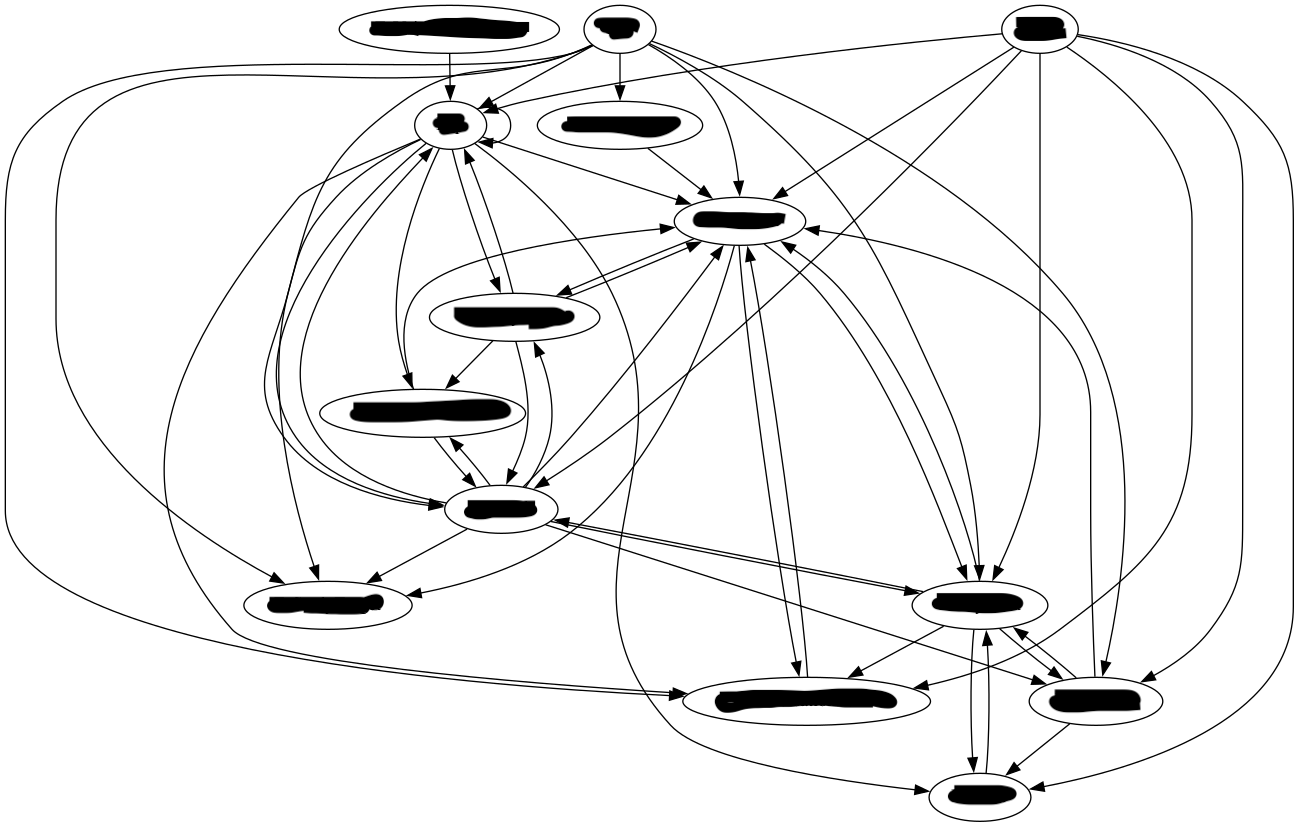
\includegraphics[width=\columnwidth]{img/graph.png}
        \caption{Very complicated micro services}
        \label{fig:graph}
      \end{figure}
    \end{column}
  \end{columns}

  \note{
    \begin{itemize}
      \item 我々はスタディーサプリENGLISHというプロダクトを開発していて、
      ソースコード規模としては3月時点でテスト込みで87万行ある。
      protobufやgRPCで生成されたコードを含めると100万行以上となる

      \item 図\ref{fig:graph}にあるようにマイクロサービスの数も多く、関係も複雑となっている

      \item こういうものを16名程度のメンバーで維持するとなると、今回紹介したdatatype generic programmingや
      他にもscalafixといったメタプログラミングのテクニックはとても重要となる
    \end{itemize}
  }
\end{frame}

\section*{References}
\begin{frame}%[allowframebreaks]
  \frametitle{References}
  % \nocite{*}
  \bibliographystyle{junsrt_url}
  \bibliography{ref}
\end{frame}

\begin{frame}
  \centering
  {\Huge Thank you for the attention!}
\end{frame}

\end{document}
